\documentclass[tikz,border=2pt]{standalone}
\usepackage{amsmath,amssymb}
\usepackage{tikz}
\usetikzlibrary{arrows.meta}

\begin{document}
% ε-δ in metric spaces: for the target ball of radius ε around f(x0) there is a ball of radius δ
% around x0 whose image lands inside it.
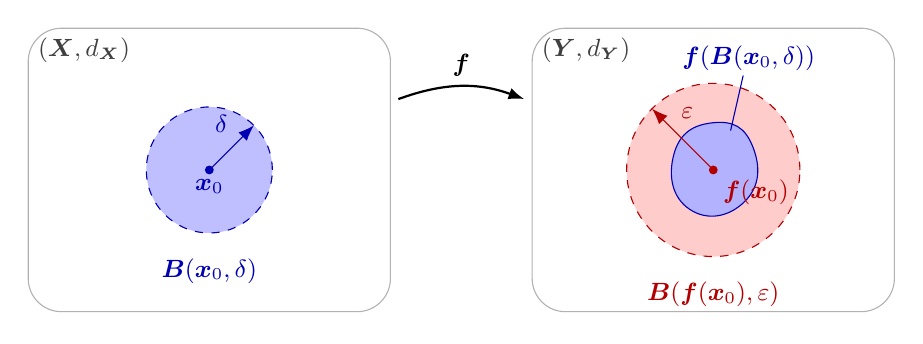
\begin{tikzpicture}[every node/.style={font=\small}, >={Latex[length=2mm]}]
	\draw[gray!60, rounded corners=12pt] (-2.3,-1.8) rectangle (2.3,1.8);
	\node[gray!50!black, anchor=north west] at (-2.3,1.8) {$(\boldsymbol{X},d_{\boldsymbol{X}})$};
	\fill[blue!25] (0,0) circle (0.8);
	\draw[blue!70!black, dashed] (0,0) circle (0.8);
	\fill[blue!70!black] (0,0) circle (1.6pt) node[below] {$\boldsymbol{x}_0$};
	\draw[->, blue!70!black] (0,0) -- (45:0.8); \node[blue!70!black] at (45:0.5) [above left] {$\delta$};
	\node[blue!70!black, anchor=north] at (0,-1.0) {$\boldsymbol{B}(\boldsymbol{x}_0,\delta)$};
	\begin{scope}[xshift=6.4cm]
		\draw[gray!60, rounded corners=12pt] (-2.3,-1.8) rectangle (2.3,1.8);
		\node[gray!50!black, anchor=north west] at (-2.3,1.8) {$(\boldsymbol{Y},d_{\boldsymbol{Y}})$};
		\fill[red!20] (0,0) circle (1.1);
		\draw[red!70!black, dashed] (0,0) circle (1.1);
		\fill[blue!30, draw=blue!70!black] plot[smooth cycle, tension=0.9] coordinates {(-0.5,0.2) (0,0.6) (0.5,0.3) (0.4,-0.4) (-0.3,-0.5)};
		\fill[red!70!black] (0,0) circle (1.6pt) node[below right] {$\boldsymbol{f}(\boldsymbol{x}_0)$};
		\draw[->, red!70!black] (0,0) -- (135:1.1); \node[red!70!black] at (135:0.75) [above right] {$\varepsilon$};
		\node[red!70!black, anchor=north] at (0,-1.3) {$\boldsymbol{B}(\boldsymbol{f}(\boldsymbol{x}_0),\varepsilon)$};
		\node[blue!70!black, anchor=south, inner sep=2pt] at (0.45,1.18) {$\boldsymbol{f}(\boldsymbol{B}(\boldsymbol{x}_0,\delta))$};
		\draw[blue!70!black, thin] (0.38,1.2) -- (0.22,0.5);
	\end{scope}
	\draw[->, thick] (2.4,0.9) to[bend left=20] node[above] {$\boldsymbol{f}$} (4.0,0.9);
\end{tikzpicture}
\end{document}
